\subsection{DOP 24 Локальная  оптимизация при  компиляции  программы. Ориентированный  ациклический  граф  и  метод нумерации значений.}

\textbf{Базовым блоком} (ББ или линейным участком) называется последовательность следующих одна за другой инструкций MIR, обладающая следующими свойствами:
\begin{itemize}
    \item Поток управления может входить в базовый блок только через его первую инструкцию (т.е. в программе нет переходов в середину базового блока),
    \item Поток управления покидает базовый блок без останова или ветвления, кроме, возможно, последней инструкции базового блока.
\end{itemize}

\textbf{Локальная оптимизация} --- это оптимизация, которая выполняется в пределах одного базового блока(ББ). Возможные локальные оптимизации:
\begin{enumerate}
    \item Удаление общих подвыражений (инструкций, повторно вычисляющих уже вычисленные значения).
    \item Удаление мертвого кода (инструкций, вычисляющих значения, которые впоследствии не используются).
    \item Сворачивание констант (вычисление константных выражений).
    \item Изменение порядка инструкций, там, где это возможно, чтобы сократить время хранения временного значения на регистре.
    \item Снижение стоимости вычислений (замена более дорогих операций более дешевыми).
\end{enumerate}

\textbf{ОАГ и метод нумерации значений}

Все указанные преобразования для локальной оптимизации можно выполнить за один просмотр ББ, если представить его в виде ориентированного ациклического графа (ОАГ). 
Суть ОАГ заключается в том, что узлы, представляющие одинаковые значения, присутствуют в единственном экземпляре.

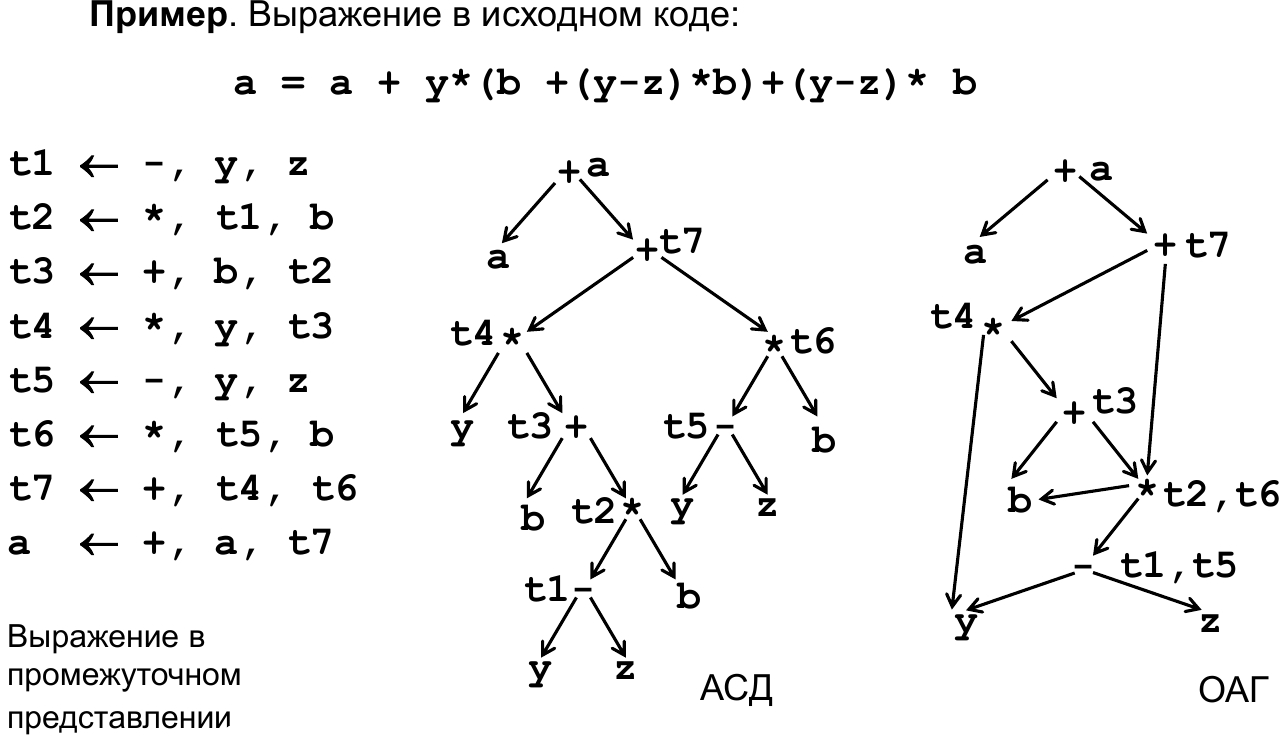
\includegraphics[width=\columnwidth]{pics/oag.png}

ОАГ можно представить в виде таблицы значений (вычислять таблицу проще для понимания). Пример таблицы ниже.

Каждая строка таблицы значений представляет один узел ОАГ. Строка содержит: 
\begin{enumerate}
    \item свой номер (номер значения)
    \item сигнатуру операции 
        \item[--] Для обычных операций \texttt{<op, \#left, \#right>}, где \texttt{ор} –-- код операции, а \texttt{\#left} и \texttt{\#right} --- номера значений левого и правого операндов (у унарных операций \texttt{\#right} равен 0)
        \item[--] Унарные операции \texttt{id} и \texttt{nm} определяют соответственно имена переменных и константы (листовые узлы). 
    \item Имена переменных, в которых хранится это значение.
\end{enumerate}

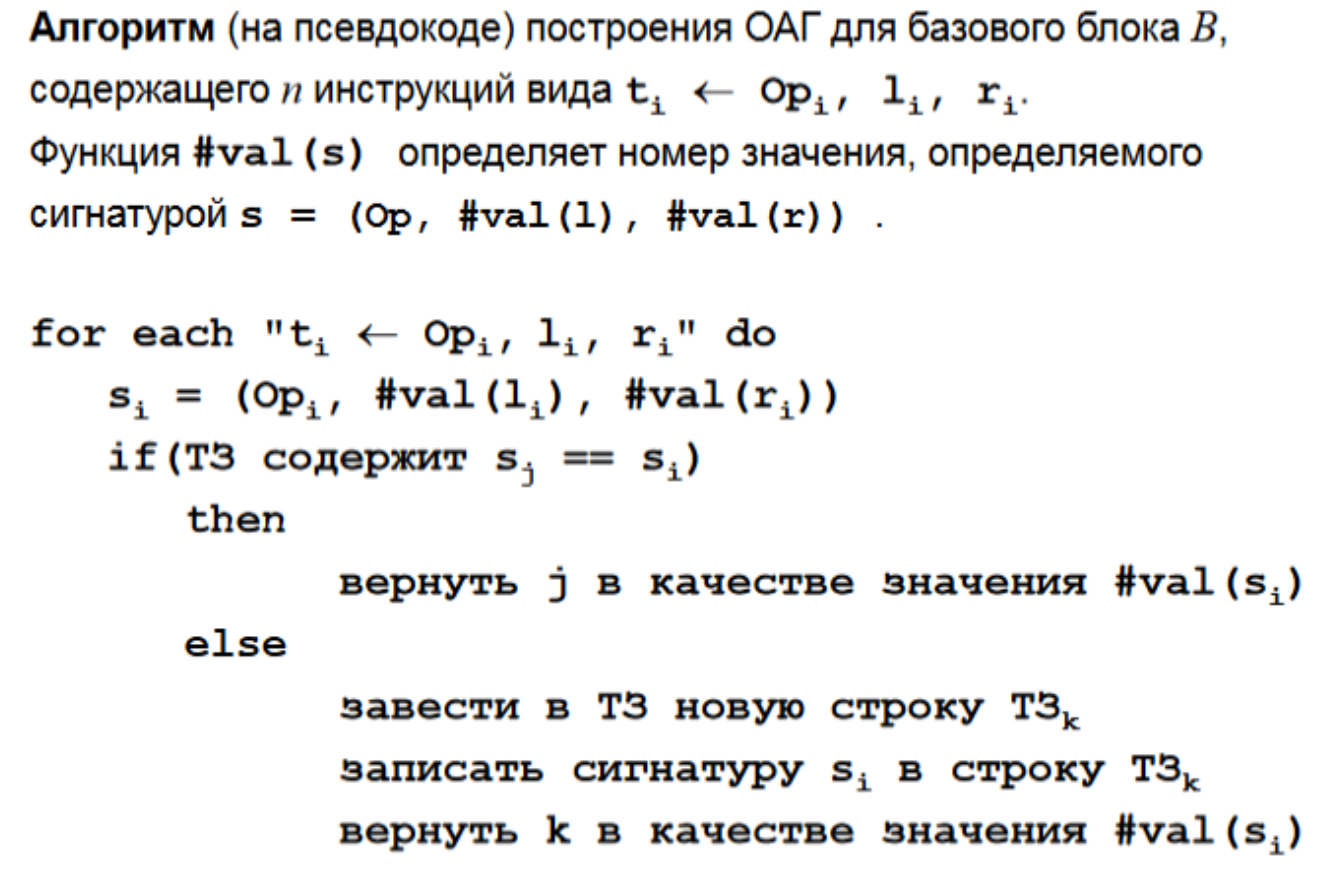
\includegraphics[width=\columnwidth]{pics/oag_alg.png}

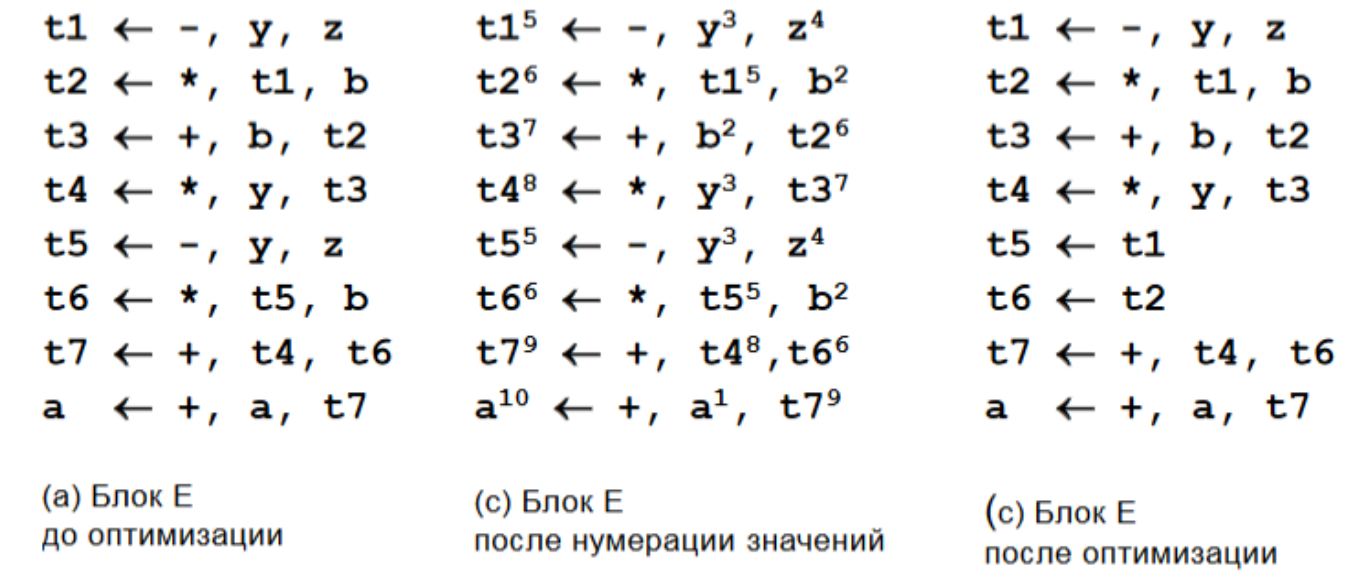
\includegraphics[width=\columnwidth]{pics/blocks.png}

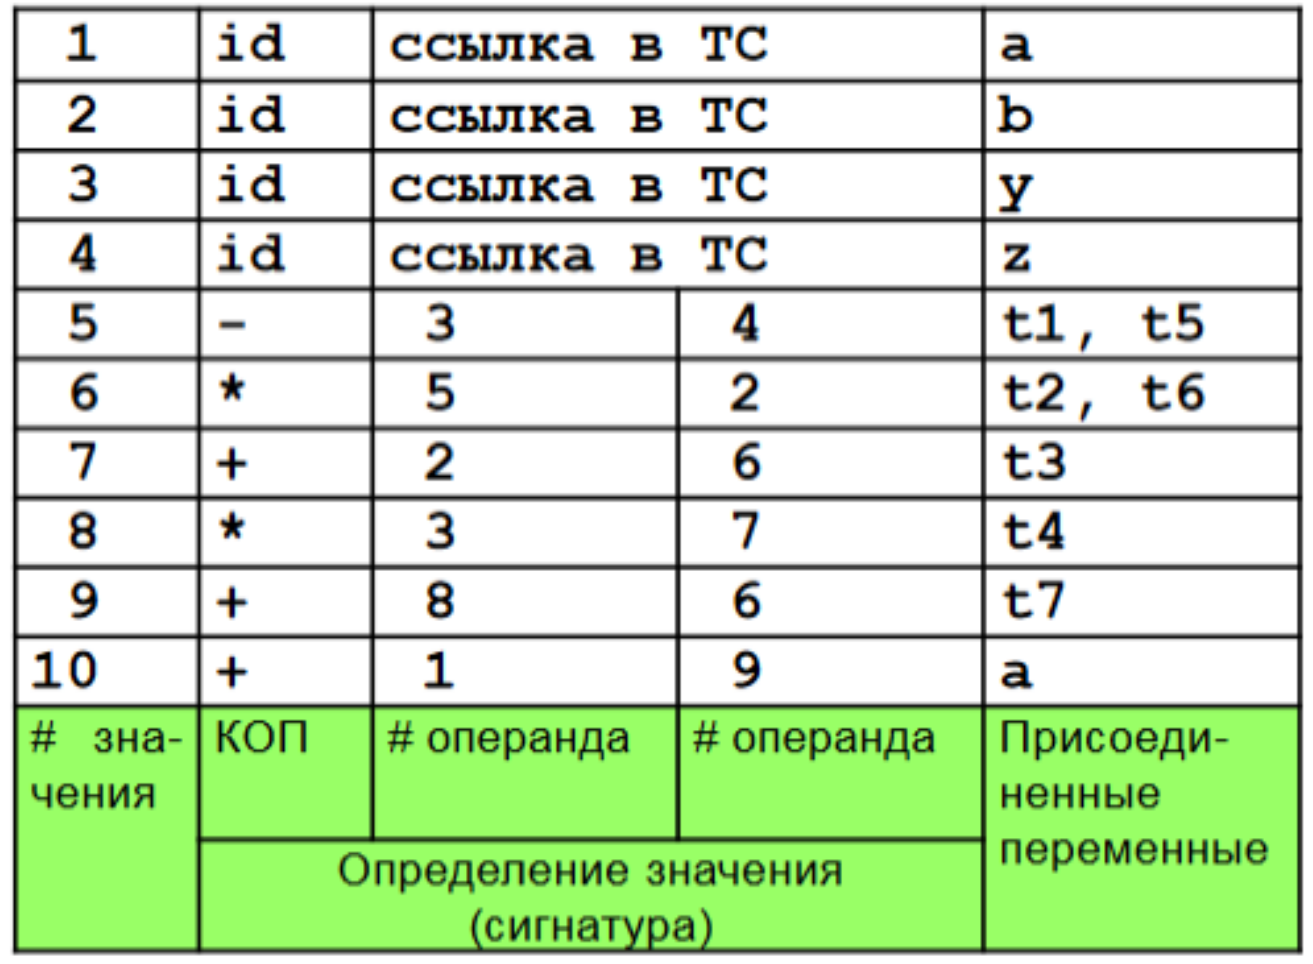
\includegraphics[width=\columnwidth]{pics/table.png}

При нумерации значений (и восстановлении базового блока из ОАГ) автоматически получаем \textit{удаление общих подвыражений}. Для значений, которым соответствуют несколько переменных достаточно вычислить одну из них, а во вторую скопировать результат.

\textbf{Сворачивание констант} также можно провести во время нумерации значений. Если оба операнда - константы, их результат можно сразу вычислить и записать в таблицу значений как константу.

\textbf{Удаление мертвого кода} --- более сложная оптимизация, которая требует знаний о других блоках. Для описания алгоритма расширим понятие базового блока

\textit{Базовым блоком} (ББ) называется тройка \textit{(B = P, Input, Output)}, где 
\begin{itemize}
    \item \textit{P} последовательность инструкций, 
    \item \textit{Input} – множество переменных, определенных до входа в блок B, 
    \item \textit{Output} – множество переменных, используемых после выхода из блока B.
\end{itemize}

\textit{Живыми} называются переменные, значения которых, вычисленные в рассматриваемом базовом блоке, используются в других базовых блоках.

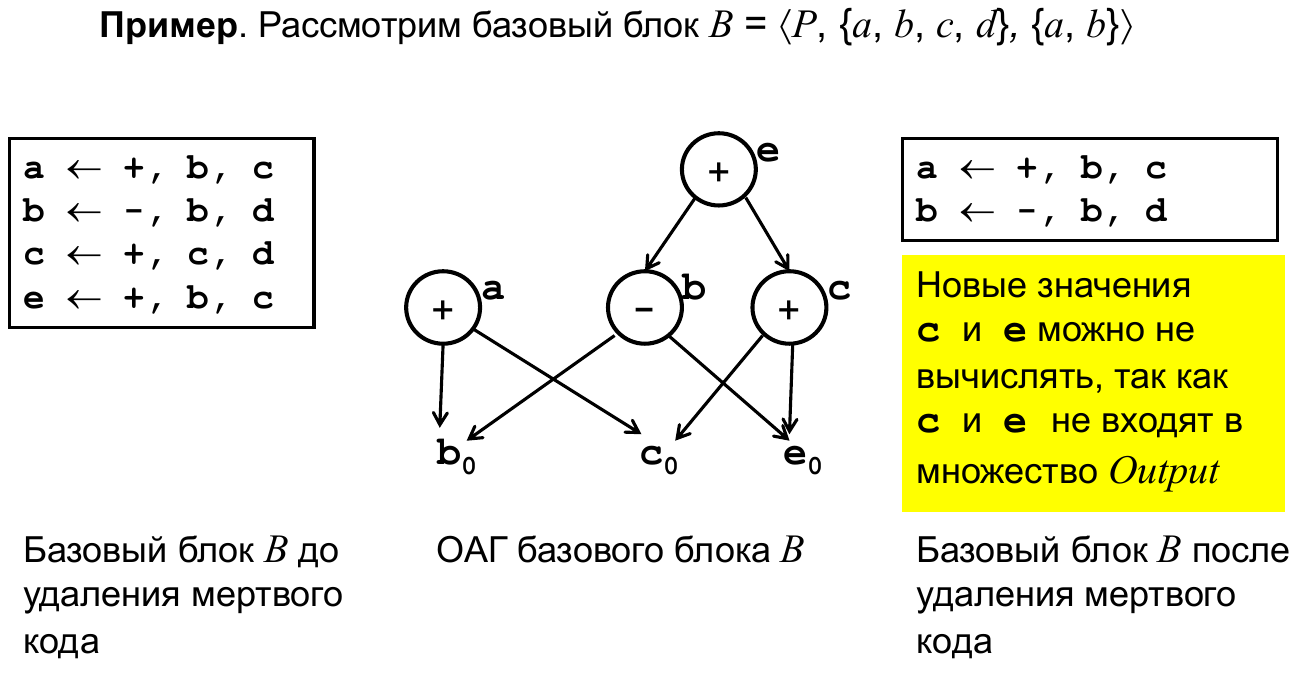
\includegraphics[width=0.8\columnwidth]{pics/dead_code.png}

\textbf{Восстановление базового блока по его ОАГ}
\begin{itemize}
    \item Для каждого узла с одной или несколькими cвязанными переменными строится трехадресная инструкция, которая вычисляет значение одной из этих переменных.
    \item Если у узла несколько присоединенных живых переменных, то следует добавить команды копирования, которые присвоят корректное значение каждой из этих переменных.
\end{itemize}

% -------- source --------
\bigbreak
[\cite[slides 29-45]{ssg}]